
\chapter{Architecture}

\section{Lexica}

\subsection{Disk Map}

To store the lexica it is necessary to use a disk-based data structure that
allows the program to quickly and efficiently seek the datum associated to a
particular key, that is an index term. To achieve this we make use of following:

\begin{itemize}
	\item to reduce disk seek time, the terms' data are compressed with
	\textit{integer compression} and the terms themselves with \textit{prefix compression}
	
	\item to minimize disk accesses, the terms are ordered lexicographically
	and partitioned in pages of the same size of the disk's page
	
	\item terms at the beginning of each page are stored in a separated array that fits in system memory, to quickly locate --- through \textit{binary search} or a \textit{trie visit} --- in which page a given term is located
\end{itemize}

\paragraph{Structure}
Let us call $|B|$ the size of a disk page, $|T|$ the maximum length off all terms stored, $m$ the maximum number of key-value pairs stored in a page, $k$ the number of pages used to store them all, $s_1 > s_2 > s_3 > \dots$ the terms to store and $d_1, d_2, d_3, \dots$ their data; and $s_{b_1} > s_{b_2} > \dots > s_{b_k}$ the terms that appear at the start of each page.

The following picture shows how our data are organized at high level

\begin{figure}[H]
	\centering
	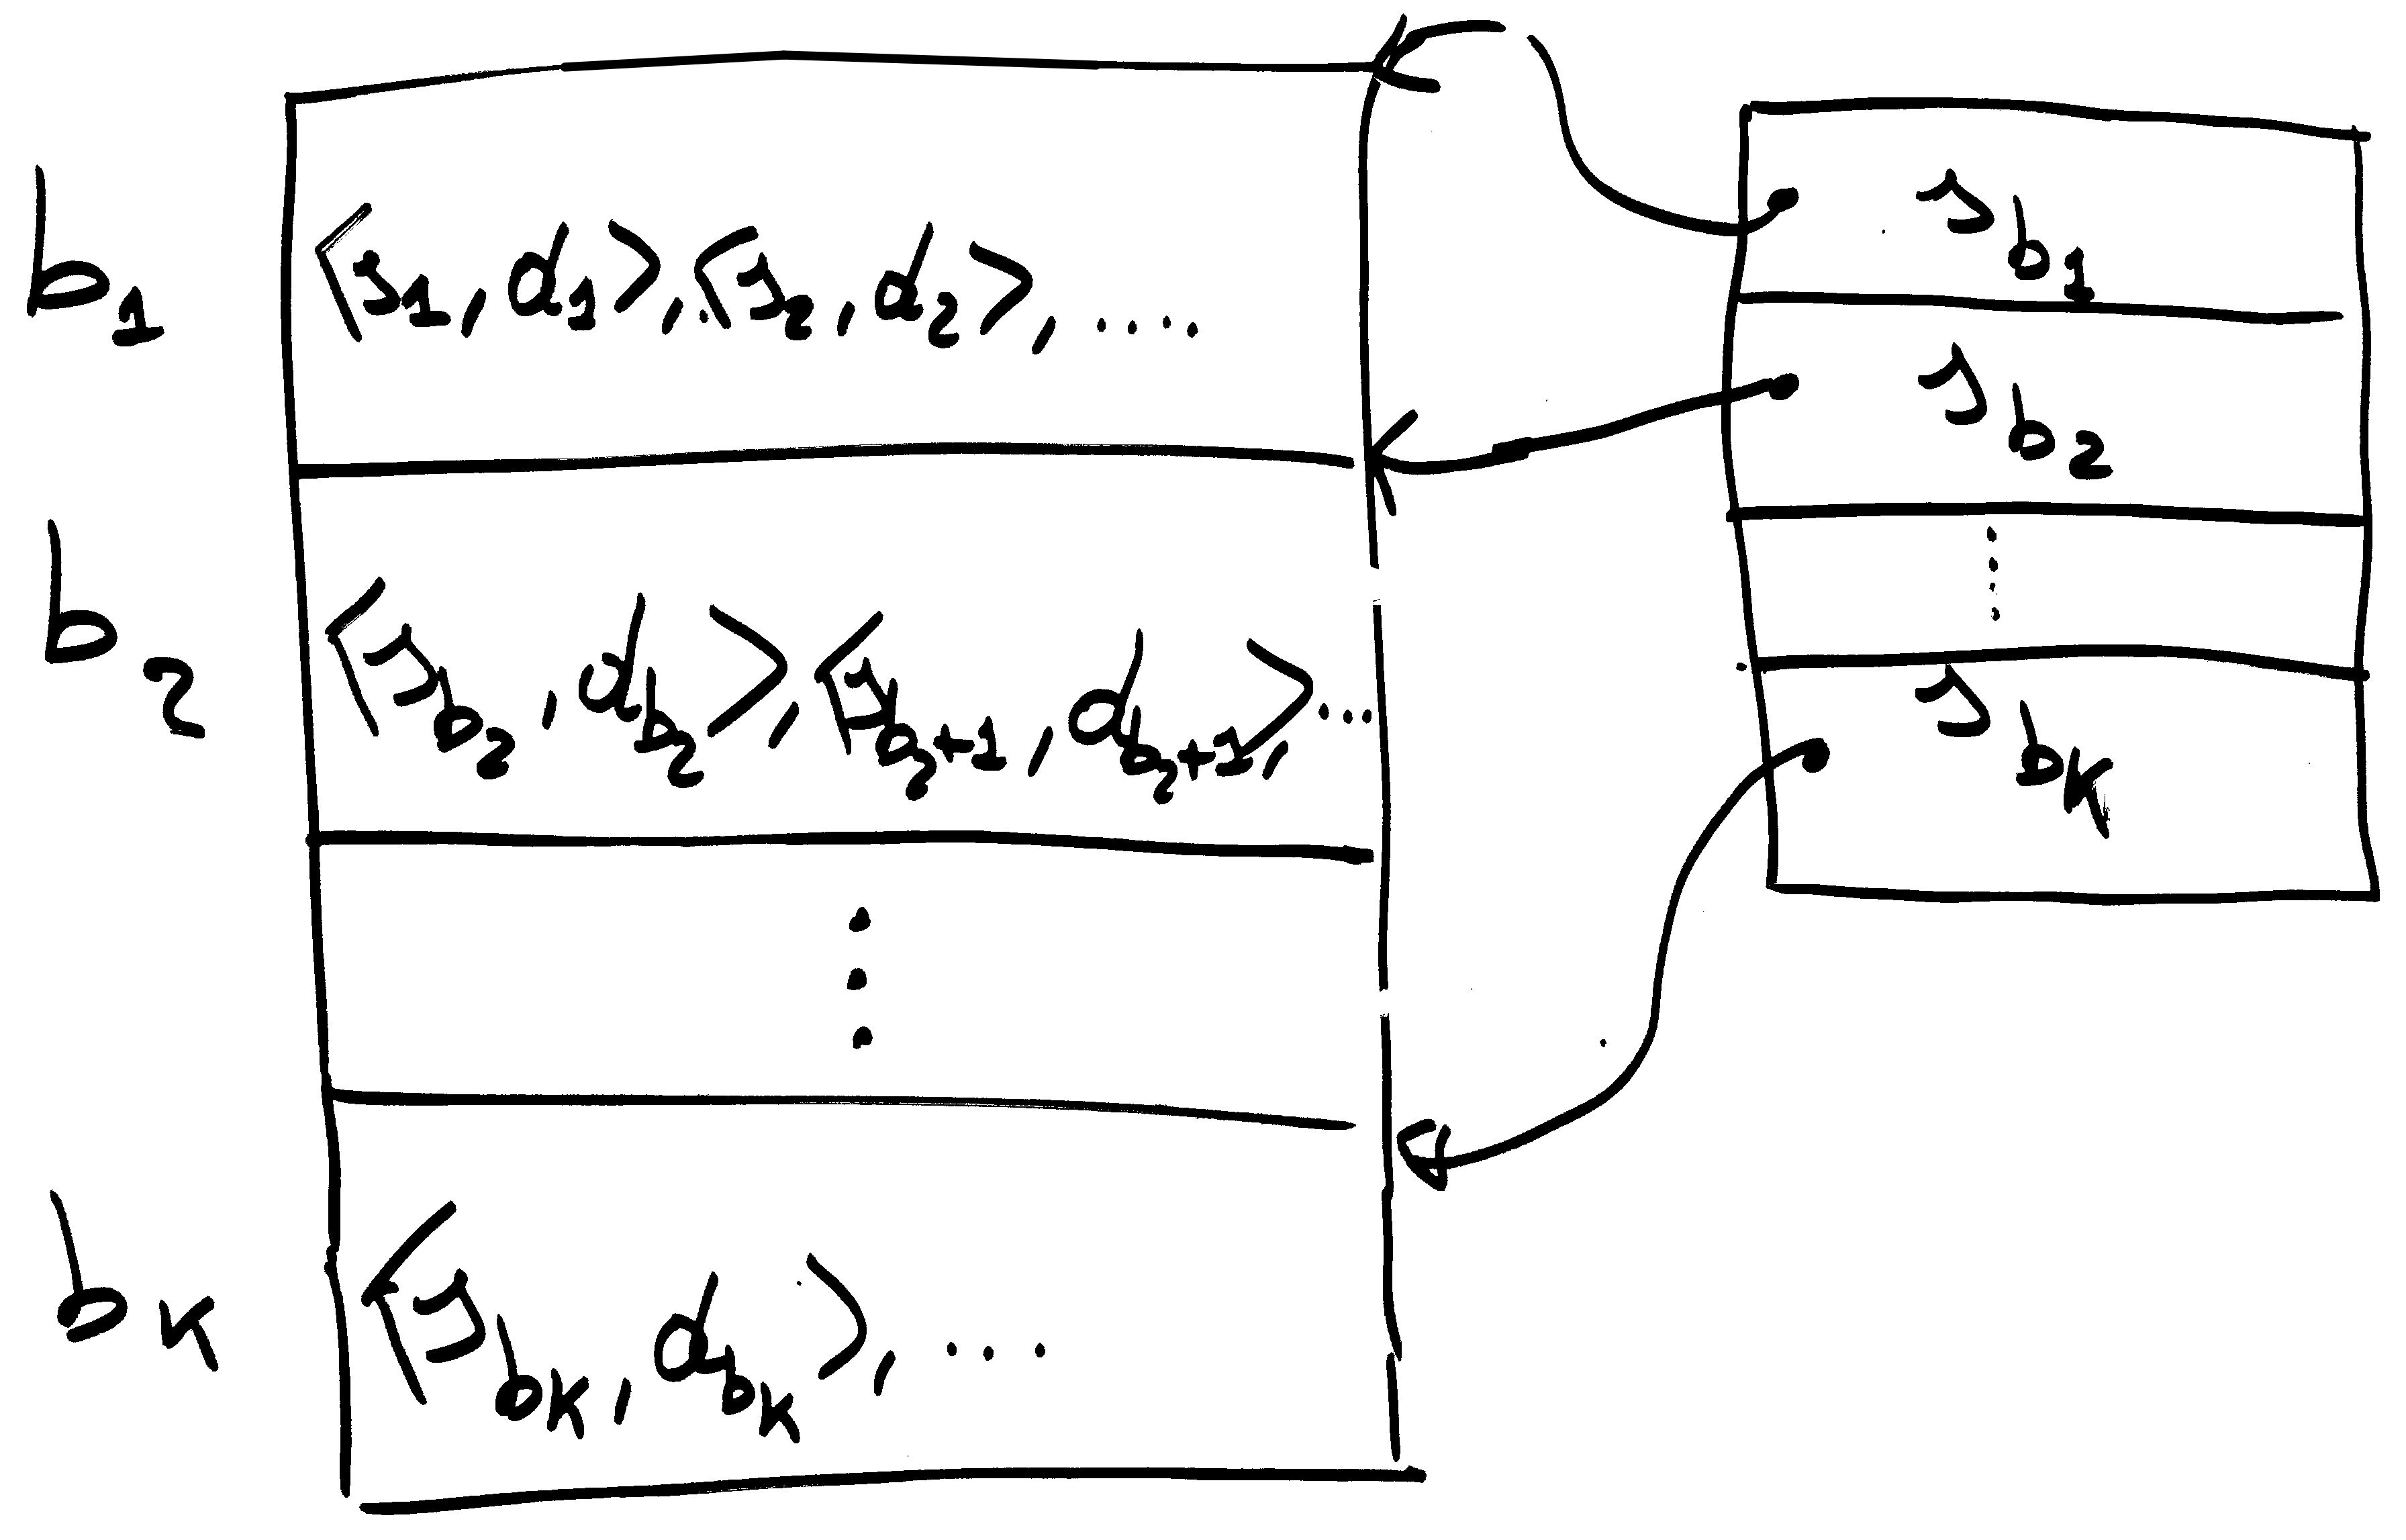
\includegraphics[width=0.6\linewidth]{assets/disk_map_base}
	\caption[]{Data organization}
	\label{fig:diskmapbase}
\end{figure}

In the real implementation, the pages' term heads $s_{b_i}$ are only stored in the look-up table, the data $d_i$ are compressed using \textit{variable bytes} and the other strings $s_j$ are compressed by cutting the common prefix they've with the page's head, so a generic key-value pair is more like:
$\left<	\left< p(s_{b_i}, s_j), {s'}_j \right>, c(d_j)	\right>$; where $p()$ is the length of the common prefix, $ {s'}_j$ is the string without the common prefix, and $c(d_j)$ is the compressed datum. The prefix's length is stored on a eight bit unsigned number, thus allowing for a maximum term's length of 255 bytes.

\paragraph{Complexity}
For simplicity's sake our implementation makes use of binary search to find in which page a term is stored and a linear scan to find it in the page, giving us a time complexity of 
$O\left(	|T|\cdot\log(k) + m	\right)$,
a space complexity, with regard to system memory, of
$O\left(	|T|\cdot k	\right)$
--- since we only have to keep the heads in memory --- and an I/O complexity of
$O\left(	1	\right)$, assuming all pages' heads fit in memory.

\subsection{Data}

\paragraph{Local lexica}
Each local lexicon stores the terms' information as \texttt{LexiconValue} during the first pass and then as \texttt{SigmaLexiconValue} in the second pass, when the upper bounds are computed and the skipping lists built.

Both structures store the number of docs in which such term appears and pointers to the compressed term frequencies and documents' ids. The latter structure also contains the skipping list and the upper bounds for \textit{TFIDF} and \textit{BM25}.

\paragraph{Global lexicon}
The only global lexicon just stores the total number of documents each term appear in, this is necessary to correctly compute the \textit{IDF} term.

